%%%% Proceedings format for most of ACM conferences (with the exceptions listed below) and all ICPS volumes.
\documentclass[sigconf]{acmart}
\settopmatter{printacmref=false} % Removes citation information below abstract
\renewcommand\footnotetextcopyrightpermission[1]{} % removes footnote with conference information in first column
\pagestyle{plain} % removes running headers
%%%% As of March 2017, [siggraph] is no longer used. Please use sigconf (above) for SIGGRAPH conferences.

%%%% Proceedings format for SIGPLAN conferences 
% \documentclass[sigplan, anonymous, review]{acmart}

%%%% Proceedings format for SIGCHI conferences
% \documentclass[sigchi, review]{acmart}

%%%% To use the SIGCHI extended abstract template, please visit
% https://www.overleaf.com/read/zzzfqvkmrfzn

\usepackage{booktabs} % For formal tables
\usepackage{graphicx}

% Copyright
%\setcopyright{none}
%\setcopyright{acmcopyright}
%\setcopyright{acmlicensed}
\setcopyright{rightsretained}
%\setcopyright{usgov}
%\setcopyright{usgovmixed}
%\setcopyright{cagov}
%\setcopyright{cagovmixed}


% DOI
%\acmDOI{10.475/123_4}

% ISBN
%\acmISBN{123-4567-24-567/08/06}

%Conference
%\copyrightyear{2017}

%\acmPrice{15.00}


\begin{document}
\title{Face Recognition using Space Variant Sensors}

\author{Pranav Sodhani}
\affiliation{%
  \institution{University of California, Los Angeles}
}
\email{sodhanipranav@cs.ucla.edu}

\author{Atishay Aggarwal}
\affiliation{%
  \institution{University of California, Los Angeles}
}
\email{atishay5395@cs.ucla.edu}

\author{Shikhar Malhotra}
\affiliation{%
  \institution{University of California, Los Angeles}
}
\email{smalhotra@cs.ucla.edu}

\author{Ameya Kabre}
\affiliation{
  \institution{University of California, Los Angeles}
}
\email{akabre@ucla.edu}

\author{Pranav Thulasiram Bhat}
\affiliation{%
  \institution{University of California, Los Angeles}
}
\email{pranavtbhat@ucla.edu}



\begin{abstract}
Human Visual System (HVS) has evolved exceptionally well when it comes to the task of face recognition. In order to develop artificial vision systems with human-like
ability of detecting and identifying faces, a lot of research has been done since the last 2 decades at the intersection of machine learning and image processing. However, although the goal has been to match human like performance for face recognition tasks, the approaches followed have been quite disparate.Traditional face recognition algorithms assume the existence of an N x M rectangular image and the presence of a Cartesian grid defining the image structure. In such architectures, resolution (density of pixels per unit area) is uniform across the image. On the other hand, most biological vision systems deploy a space variant sampling with a higher concentration of photoreceptors in the fovea while diminishing concentration towards the periphery. This allows such systems to work with significantly
lower bandwidth while still maintaining a high acuity of the visual scene at the fovea. Inspired by human visual system, in this paper, we adopt a biologically plausible
approach towards the problem of face-recognition system and, to that end, propose and implement algorithms for such tasks. Results obtained using 2 popular face databases show that space variant sensors, even when applied in a straight-forward manner, do not lag traditional image processing algorithms by a big margin for the task of face recognition.
\end{abstract}

%
% The code below should be generated by the tool at
% http://dl.acm.org/ccs.cfm
% Please copy and paste the code instead of the example below. 
%
%\begin{CCSXML}
%<ccs2012>
% <concept>
%  <concept_id>10010520.10010553.10010562</concept_id>
%  <concept_desc>Software Engineering ~ Malware detection</concept_desc>
%  <concept_significance>500</concept_significance>
% </concept>
% <concept>
%  <concept_id>10010520.10010575.10010755</concept_id>
%  <concept_desc>Software Engineering~piracy detection</concept_desc>
%  <concept_significance>300</concept_significance>
% </concept>
%</ccs2012>  
%\end{CCSXML}

%\ccsdesc[500]{Computer systems organization~Embedded systems}
%\ccsdesc[300]{Computer systems organization~Redundancy}
%\ccsdesc{Computer systems organization~Robotics}
%\ccsdesc[100]{Networks~Network reliability}

% We no longer use \terms command
%\terms{Theory}

\keywords{Human Visual System, face recognition, machine learning, Cartesian grid, biological vision, photoreceptors, fovea}

%% Used in some conference proceedings e.g. sigplan and sigchi
% \begin{teaserfigure}
%   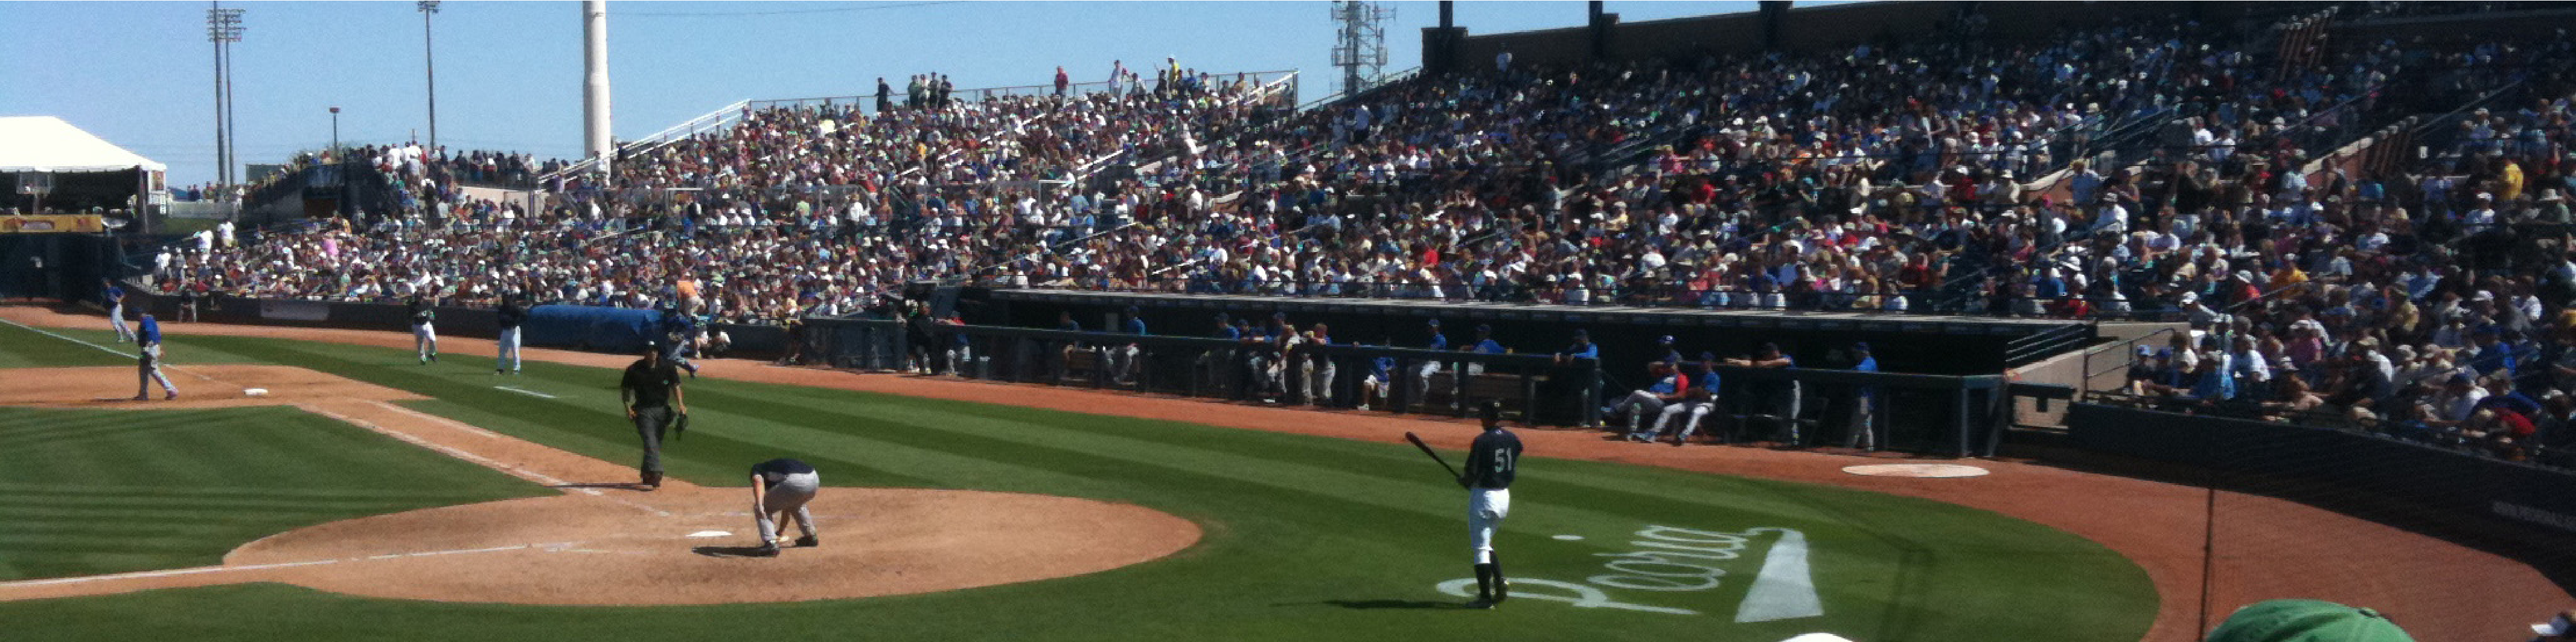
\includegraphics[width=\textwidth]{sampleteaser}
%   \caption{This is a teaser}
%   \label{fig:teaser}
% \end{teaserfigure}

\maketitle

\section{Introduction} \label{introduction}
In recent years, with the emergence of fields such as surveillance, biometrics and tracking systems, face recognition technology has received significant attention. Given the complexity of the problem, a lot of approaches have been proposed in the literature which take different routes to address it \cite{ramkumar2013face}. At the same time, the tremendous visual processing capability of humans has fascinated both biologists and computer scientists.

Robust computational models of face recognition are interesting not only because they contribute to theoretical insights but also to practical computer applications such as film processing, human-computer interaction, criminal tracking and security systems. Human visual system has evolved exceptionally well to detect faces even in complex settings. For example, even under different illumination conditions, different poses, different expressions and at different scales, humans can easily both detect as well recognize faces of many individuals. On the other hand, even the most complex algorithms such as deep neural networks have failed to provide human like accuracy. As such, it is totally reasonable to adopt a biologically inspired vision system which is far less complex and at the same time more robust when it comes to the task of face recognition.

Traditionally, images have been represented as an N x M grid of pixels. Such representations assume the presence of a Cartesian grid and thus defining pixel neighborhood is easy. Also, the density of pixels in uniform across the image. On the other hand, images formed in our retina are quite different. The density of photo-receptors is the highest at the fovea located at the center of the retina and decreases gradually towards the periphery. This gives humans the ability to focus at things which are important, while also maintaining a relatively blurred view of the surrounding. Active vision models can hugely benefit from such models since a broader view can be maintained while processing at a significantly lower bandwidth. 
 
In this paper, we adapt traditional face recognition algorithms to a space-variant setting. Specifically, we modify 3 well known approaches - PCA, ICA and LDA and show how space variant models can utilize these techniques for face recognition. Since neural network based models have recently outperformed all earlier approaches, we also show a neural network based based on space variant images for face recognition. 
In summary, the paper makes the following contributions:
\begin{itemize}
\item We demonstrate how algorithms like Eigenfaces \cite{eigenfaces}, Independent Component Analysis \cite{bartlett2002face} and Fisherfaces \cite{etemad1997discriminant} can be applied for face recognition in space variant sensors. Using the ORL face database \cite{orl} , we evaluate performance of the proposed algorithms
\item A neural network based face-recognition is being presented which works for space-variant sensors.
\item Finally, in order to address the challenge of illumination-invariance, we adapt a robust illumination invariance technique in the setting of space variant sensors and demonstrate its performance on the Yale Face Database B \cite{yale}
\end{itemize}

\begin{figure*}[t]
\centering
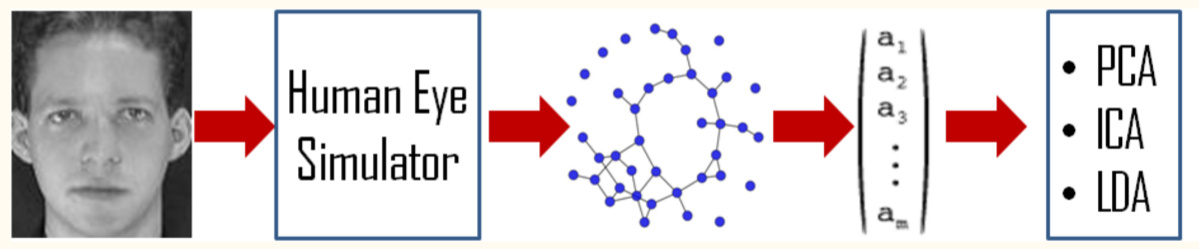
\includegraphics[height=1in, width=\textwidth, trim={0 0.3cm 0 0},clip]{flowchart1.jpg}
\caption{Adaptation of traditional algorithms to a space-variant setting}
\vskip -6pt
\label{fig:flowchart1}
\end{figure*}

The rest of the paper is organized as follows. Section \ref{relatedwork} presents a complete study of different approaches proposed in the literature towards face recognition. We cover all major traditional algorithms proposed in the literature and also throw light on approaches similar to ours. In section \ref{approach}, we propose and describe the implementation of different space-variant algorithms and show how we overcome the challenge of illumination invariance. Section \ref{evaluation} presents evaluation results obtained on 2 popular face datasets. Finally, \ref{futconc} concludes the paper and presents future work.

\section{Related Work} \label{relatedwork}
Face recognition has a wide range of applications in the fields of biometrics (authentication systems), surveillance (person tracking) and entertainment (VR and video games). Given the huge base of stakeholders, research on face recognition has gained a lot of focus over the last few years \cite{jafri2009survey}. These algorithms can be broadly classified as belonging to 2 classes - shallow algorithms, which either extract features or match templates for calculating a similarity score between faces and deep algorithms, which deploy neural networks for face identification. Eigenfaces using principal component analysis (PCA) \cite{eigenfaces}, one of the most popular algorithms for face recognition, uses KL transform to reduce the dimensionality of images while retaining most discriminating features. A nearest neighbor approach then helps find the closest matching face. PCA based algorithms are, however, not robust to pose and illumination changes. In \cite{vasilescu2002multilinear}, Vasilescu et al. develop a multi-linear algebraic framework to extend PCA and make it pose and illumination variant. Such algorithms, however, require the presence of huge training sets for better performance. Images may contain higher order statistical data present in their pixels. An improved algorithm, Independent Component Analysis (ICA) was proposed to find such basis images using the principle of optimal information transfer through sigmoidal neurons. ICA tries to minimize both second-order and higher-order dependencies in the input data and finds the basis along which the image data is statistically independent. Bartlett et al. \cite{bartlett2002face} discussed two such architectures. While the first one - statistically independent basis images attempts to discover a spatially local basis for the faces in the images, the second one produces a factorial face code. Performance evaluation demonstrates it to be a better technique than PCA. When both the architectures are combined together, optimal results are obtained. 

Parkhi et al. \cite{parkhi2015deep}, extensively describe face recognition techniques using Convolutional Neural Networks or CNNs. The key to developing a good classifier, according to the authors, is to develop a deep network i.e., one having several layers. The face recognition problem is first modeled as a N-way classification problem, where N is the number of distinct people in the dataset. During the learning phase, the CNN develops a score vector, using a fully connected “classifier” layer. The scores are compared to the ground truth classes by computing the softmax log-loss. Then, the fully connected classifier layer is removed, and the generated scores for each testing image are classified by simply picking the class with the minimum Euclidean distance. The performance of the classifier can be improved further by learning embeddings for score vectors. The authors describe this scheme to be “triplet-loss training”.

To the best of our knowledge, there has been no work done in the realm of face recognition using space variant sensors. The most similar work in this category assumes log-polar mapping sensors for the task of object detection \cite{traver2004appearance}, the authors of \cite{traver2004appearance} demonstrate that such systems have the ability of recognizing faces even at a low resolution. The idea of representing images as graphical structures instead of rectangular grids was presented by Wallace et al. in \cite{wallace1994space}. Leo Grady \cite{grady2004space} further extended the idea to develop low level image processing operations such as image segmentation and interpolation. He has also provided a MATLAB toolbox \cite{grady2003graph} for carrying out simple image operations using graph as the data structure for images which we use in out experiments.
 

\section{Our Approach} \label{approach}
\subsection{Space-Variant Image Processing}
Space-variant sampling of the visual environment is ubiquitous in higher vertebrate animals. This is attributed to the non-uniform density of ganglion cells in the retina of different species. This architecture is beneficial in computer vision because of huge reduction in space complexity. Representation of image data on graph-theoretic structures provide one way to universal sampling and visual sensing.

In this approach, we consider representing pixels as nodes of a graph where edges can be used to establish neighborhood relationships between pixels. Such a graph has high density of nodes at the center representing the fovea and decreasing number of nodes towards the periphery. Given an N x M image, we transform it to a graphical structure using the toolbox provided by Leo Grady \cite{grady2003graph}. Specifically, we specify the retinal structure of the eye and the image and get a set of nodes and edge relationships. The value stored at these nodes represent the luminance values of transformed pixels. The nodes of this graph can then be used by conventional algorithms such as PCA, LDA, ICA for further processing. Figure \ref{fig:vis1} shows the transformation of an N x M face image using a retinal structure of a kangaroo's eye. In (c) and (d), using two visualization techniques - triangulation and Voronoi cells, we show how these images look at the retina when the fixation point is the center of the image.
\begin{figure}[h]
\centering
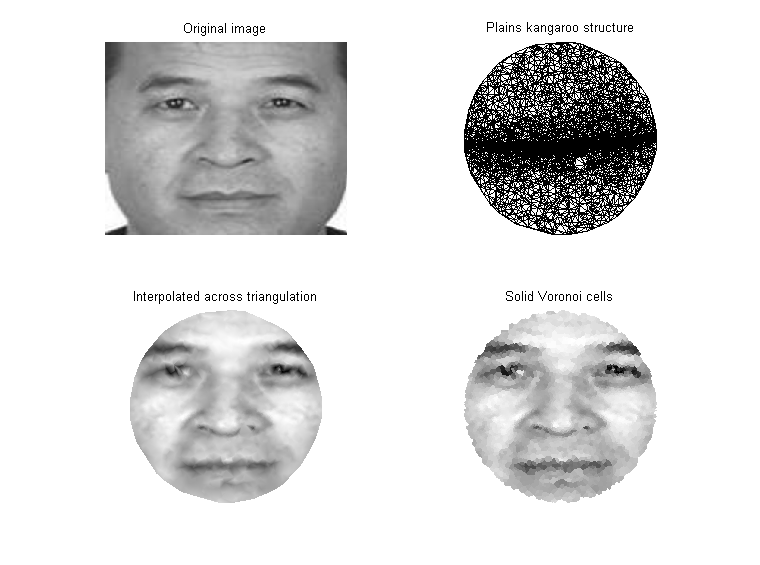
\includegraphics[height=1.5in, width=2.5in, trim={0 0.3cm 0 0},clip]{visualization_result.png}
\caption{(a) A traditional N x M face image (b) Photo-receptor organization in eyes of a kangaroo (c) Visualization using triangulation and (d) Visualization using solid Voronoi cells }
\vskip -6pt
\label{fig:vis1}
\end{figure}

\subsection{Eigenfaces based face-recognition}
Eigenfaces is an application of principal component analysis when applied to the task of representing images in a low dimensional space. Sirovich and Kirby \cite{kirby1990application} showed that PCA could be applied on a set of face images to form basis features. Thus, if we have an m-dimensional vector representation of every face in a training set of images, Principal Component Analysis (PCA) can be applied to find an n-dimensional subspace whose basis vectors correspond to the maximum variance direction in the original image space. This new subspace is normally lower dimensional (n<<m).Not only does this reduce dimensionality, it also improves accuracy by ignoring redundant features. The PCA basis vectors are defined as eigenvectors of the scatter matrix.

Traditionally, to form the m-dimensional feature vector, every row of the image is scanned and appended sequentially to form the N x M dimensional feature vector. For a space variant image, we scan the nodes in a fixed order to form the 1D feature vector which represents the image. This is then fed to a regular PCA based face recognition system. In our experiments on using the ORL database, we observe that top 25 eigenvectors are sufficient and accuracy does not increase further on increasing the number of eigenvectors.

\subsection{ICA based face recognition}
While PCA aims at finding features which represent images in a low dimensional space, Linear Discriminant analysis or LDA tries to find features which are the most discriminating across classes. Specifically, LDA aims at minimizing within-cluster distance while maximizing between-cluster distance. For all samples of all classes the between-class scatter matrix SB and the within-class scatter matrix SW are defined. The goal is to maximize SB while minimizing SW, in other words, maximize the ratio det|SB|/det|SW|, where det stands for determinant of these matrices . This ratio is maximized when the column vectors of the projection matrix are the eigenvectors of $(SW^-1 × SB)$.

LDA again requires 1D vector representation of each face image. We deploy the same technique as PCA for converting space variant images represented as graphs into 1D vectors.

\subsection{Fisherfaces based face-recognition}
While PCA aims at finding features which represent images in a low dimensional space, Linear Discriminant analysis or LDA tries to find features which are the most discriminating across classes. Specifically, LDA aims at minimizing within-cluster distance while maximizing between-cluster distance. For all samples of all classes the between-class scatter matrix SB and the within-class scatter matrix SW are defined. The goal is to maximize SB while minimizing SW, in other words, maximize the ratio det|SB|/det|SW|, where det stands for determinant of these matrices . This ratio is maximized when the column vectors of the projection matrix are the eigenvectors of $(SW^-1 × SB)$.

LDA again requires 1D vector representation of each face image. We deploy the same technique as PCA for converting space variant images represented as graphs into 1D vectors.


\subsection{Illumination-invariant face-recognition}
Humans have an innate ability to recognize faces under varying illumination conditions. One approach towards building a computational model is to train the model under varying lightning conditions. However, this is not a biological way since we do not train our eyes under different lightning conditions to recognize faces. Instead, an alternate way which is more biologically plausible is to remove the reflectance part of the image and only capture its luminance.

According to the Lambertian reflectance model, an image can be decomposed as a product of reflectance and luminance matrices. In our case, while luminance captures the properties of a face, reflectance captures information about surrounding light. Since we are interested in recognizing faces, we need to work only with the luminance matrix.
Wang et al. \cite{sqi} introduced the concept of Self Quotient Image for addressing the issue of illumination invariance using only a single face image. They represent the luminance matrix as a quotient image obtained by ratio of the original image and its smoothened version. The smoothened version of an image is obtained using Gaussian filtering. 

It is easy to define Gaussian filtering in a traditional N x M rectangular image since neighborhood relationships are well defined. For the graphical structure we adopt, we use nodes connected via edges as neighboring nodes and perform Gaussian weighted filtering to simulate the generation of luminance matrix. Once we have the the luminance image (quotient image), we can use this directly in all models discussed above. Figure \ref{fig:illum} shows the transformation obtained after applying Gaussian filtering and obtaining the quotient image. Specifically the image at the right bottom is the quotient image of the image at the top right. 

\begin{figure}[h]
\centering
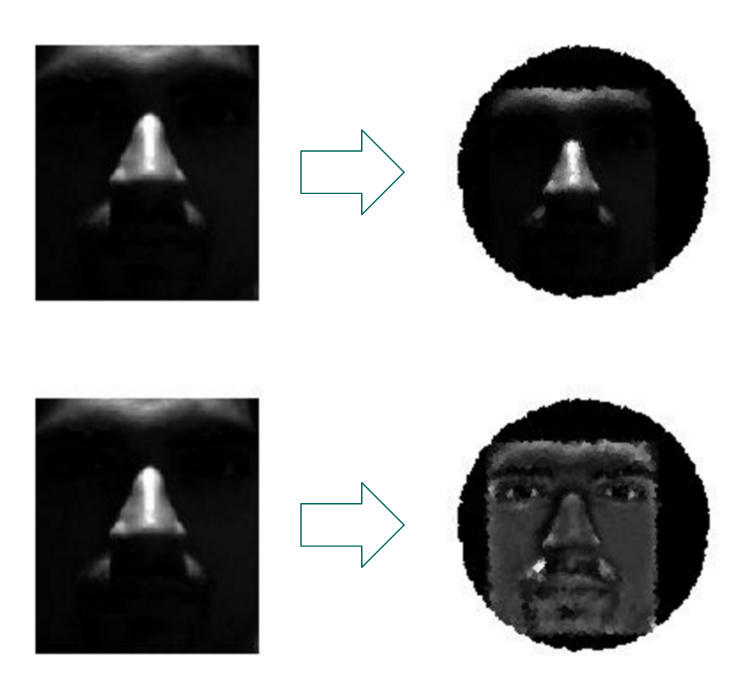
\includegraphics[height=1.5in, width=2.5in, trim={0 0.3cm 0 0},clip]{illum.jpg}
\caption{Demonstrating illumination invariance for face recognition}
\label{fig:illum}
\end{figure}

\begin{figure*}[t]
\centering
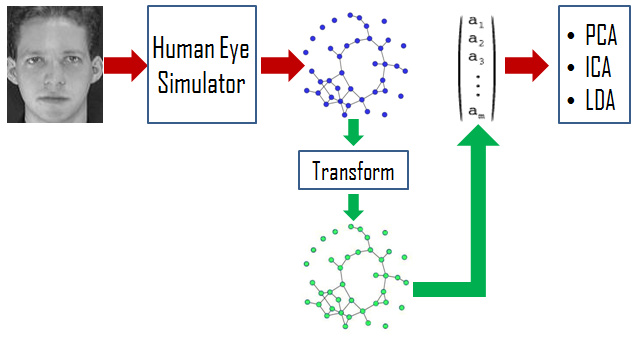
\includegraphics[height=2.0in, width=\textwidth, trim={0 0.3cm 0 0},clip]{flowchart2.jpg}
\caption{Introducing illumination invariance property transformation to the graphical structure}
\vskip -6pt
\label{fig:flowchart2}
\end{figure*}

\subsection{Neural network based face-recognition}
In this section we describe our efforts in realizing a neural-network based classifier for face recognition. We applied the same dataset preparation techniques as the other classification techniques (PCA/ICA/LDA) and passed the processed images into the Leo-Grady toolbox to obtain a feature vector for each of the images. 

We then proceeded to prepare a training and testing dataset, by associating with each feature vector its class label. These datasets were passed into a Neural Network with 10 hidden layers. Our train to test ratio was 50:50. The trained neural network is then used to classify images. We noticed that for space variant detection, the NN based classification scheme produced the best results. 


\section{Evaluation} \label{evaluation}
\subsection{Datasets Used}
We make use of 2 popular face databases - The ORL database and the Yale B database for performance evaluation. The ORL database (also known as "The Database of Faces") consists of 10 different images of 40 subjects For some subjects, the images were taken at different times, varying the lighting, facial expressions (open / closed eyes, smiling / not smiling) and facial details (glasses / no glasses). All the images were taken against a dark homogeneous background with the subjects in an upright, frontal position (with tolerance for some side movement). 

The Yale B database consists of 60 images of 38 different subjects with varying facial expressions. More importantly, all images have been taken under different illumination conditions which is the reason why we chose this database for evaluating the performance of our illumination-invariance tool. In our experiments, we use a cropped face version of the database since we do not employ face detection as a pre-processing step. 

\begin{figure}[h]
\centering
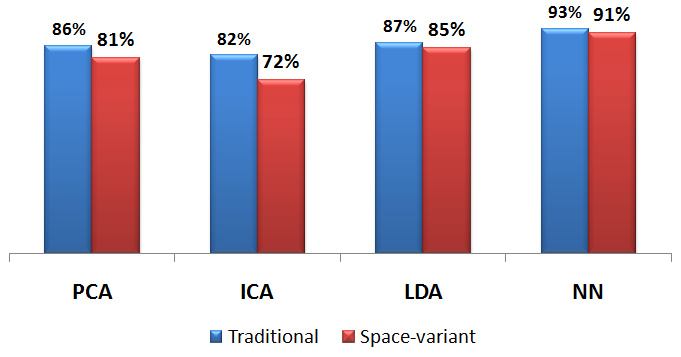
\includegraphics[height=1.5in, width=2.5in, trim={0 0.3cm 0 0},clip]{results4.jpg}
\caption{Accuracy obtained on the ORL database (Also known as "The Database of Faces")}
\vskip -6pt
\label{fig:results1}
\end{figure}

\subsection{Results and Discussions}
We distributed the ORL dataset into training and testing dataset with a 50:50 ratio, as suggested in the literature. For classification, we use the nearest neighbor approach by calculating Euclidean distance between vector representation of images. Then, we report the classification accuracy as a measure to evaluate performance of different algorithms. Figure \ref{fig:results1} shows the classification accuracy obtained using each of the 4 algorithms - PCA, ICA, LDA and Neural Network both for traditional algorithms and space-variant algorithms. It can be seen that although each of the 4 algorithms perform poorly than their traditional counterpart, yet the difference isn't high. Among all of them, neural network based model performs the best with an accuracy of 91\%.

Figure \ref{fig:results2} shows the performance on Yale B database when we use the illumination invariance tool proposed in the above section. The database is divided into 10:90 train-test ratio, as suggested in the literature. Since PCA and LDA performed much better than ICA, we decided to test the performance of only PCA and LDA. After calculating classification accuracy, we observe that LDA performs much better than PCA and space-variant counterpart for LDA performs almost the same as its traditional counterpart.
\begin{figure}[h]
\centering
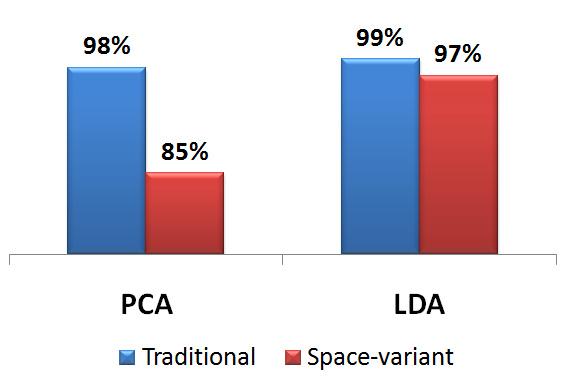
\includegraphics[height=1in, width=2.5in, trim={0 0.3cm 0 0},clip]{results3.jpg}
\caption{Accuracy obtained on the ORL database (Also known as "The Database of Faces")}
\vskip -6pt
\label{fig:results2}
\end{figure}


\section{Conclusion and Future Work} \label{futconc}
In this paper, we adopt a biologically inspired approach towards face recognition and propose algorithms for the same. Specifically, we show how existing algorithms can be tweaked to make them work in space variant setting. Initial results are encouraging since such algorithms only perform slightly worse than traditional algorithms at a significantly reduces complexity. We also address the challenge of illumination invariance, a major obstacle in face-recognition. In future, we would like to address other prominent challenges such as rotation and scale invariance. Also, a face-detection model needs to be in place to carry out the task of face recognition. Finally, using multiple fixation points on faces can be one direction in which face recognition accuracy can be improved over traditional algorithms.

\bibliographystyle{plain}
\bibliography{bibliography.bib}
\end{document}
